%Background body
%Created MS 05-11

\section{Background}\label{background}

\subsection{Optical Pumping}

Optical pumping is the process in which the interaction of light with
atoms produces a population of energy levels that is distinct from the
thermal equilibrium Boltzmann distribution \cite{bernheim}. In a
three-state system, with a ground state $|g\rangle$, excited state
$|e\rangle$, and intermediate metastable state $|m\rangle$
(Fig. \ref{blah}), it is possible to selective populate the metastable
state if the natural decay time $\gamma$ is sufficiently long in
comparison to the pumping time. If laser light is applied on resonance
with the $|e\rangle$ - $|g\rangle$ transition, it drives the atom
population to the excited state, and then the atoms decay to the lower
energy levels with some time constant. If the laser light cannot
excite atoms from the metastable state to the excited state (for
example, due to selection rules), the process preferentially populates
the state $|m\rangle$, resulting in optical pumping.


\subsection{Rubidium System}

In this experiment, we consider an ensemble of rubidium atoms as an
optical pumping system. Rubidium is an alkali atom with a single
electron in its outer shell, and thus can be modelled as a
hydrogen-like system. Here, we take the outer $5^2S_{1/2}$ level as
the ground state and focus on the $D_1$ transition between the
$5^2S_{1/2}$ and $5^2P_{1/2}$ states. 

We use a natural abundance Rubidium cell for optical pumping, which
consists of $72\%$ $^{85}$Rb and $28\%$ $^{87}$Rb, so we are able to
investigate the properties of both isotopes. The energy level diagrams
are presented in Fig.~\ref{fig:8587levels}.


\begin{figure}[h]
\begin{center}
\subfigure[$^{87}$Rb energy spectrum]{\label{fig:edge-b}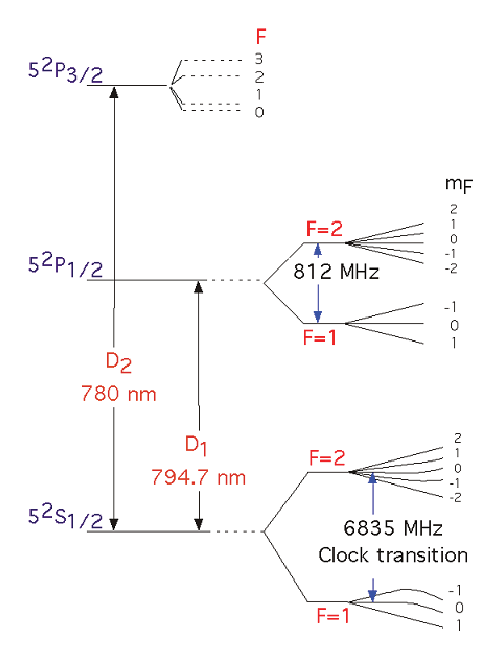
\includegraphics[height=3.5in]{figures/87levels.eps}}
\hspace{-1mm}
\vspace{-2mm}
\subfigure[$^{85}$Rb energy spectrum]{\label{fig:edge-a}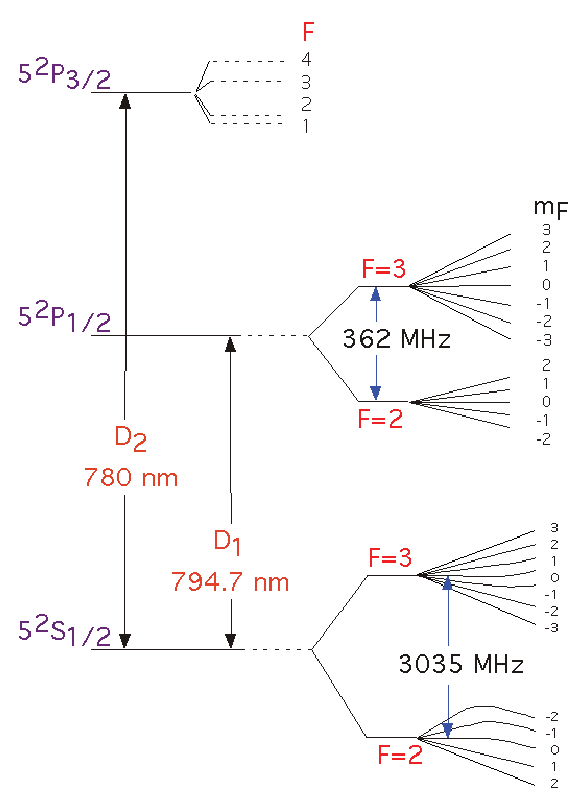
\includegraphics[height=3.5in]{figures/85levels.eps}}
\vspace{-2mm}
\caption{\small{CAPTION GOES HERE}}
\label{fig:8587levels}
\end{center}
\end{figure}

There are several levels of splitting which occur in the Rb atom. The
splitting of the $5^2P$ state into $5^2P_{1/2}$ and $5^2P_{3/2}$ is
due to spin-orbit coupling, that is, the addition of the spin and
orbital angular momenta ($S$ and $L$, respectively) of the electrion
to comprise the total angular momentum $J$. As mentioned above, the
laser has been tuned to the $D_1$ line because of its better optical
pumping properties (Fig.~\ref{fig:8587levels}).

In addition, each total electron angular momentum level is further
split by the coupling of spins of the electron to the nucleus, known
as hyperfine splitting. This results in the distinct $F$ levels, where
$F = I + J$; $I$ is the spin of the nucleus and $J$ as above is the
total electron angluar momentum. Each pair of $F$ states in these
levels of Rb is separated by a frequency shift on the order of
hundreds or thousands of MHz, allowing the tuning of the laser to a
particular transition (Fig.~\ref{fig:fluor}). For instance, we
chose to focus on the $^{85}$Rb $5^2S_{1/2}, F = 3$ to $5^2P_{1/2}, F
= 3$ transition for most of the experiment, because the density of the
$^{85}$Rb isotope is over twice as high, and the $3$ to $3$ line is
more easily separated from the neighboring transitions.

\begin{figure}[h]
\begin{center}
\includegraphics[height=3in]{figures/fluoresence.png}}
\caption{\small{Fluoresence spectrum of natural abundance rubidium. The $x$-axis is a relative measure of frequecy, with $0$ being the $D_1$ transition frequency. The dashed red line represents the fluorescence from individual transitions, and the blue line is the combined intensity.}}
\label{fig:fluor}
\end{center}
\end{figure}

Further splitting occurs in the Zeeman effect, where the degenerate
magnetic sublevels are split via an application of a uniform magnetic
field. For weak fields, the splitting is directly proportional to $B$,
the magnetic field amplitude.

\subsection{Magnetic Interactions}

\subsubsection{Zeeman Splitting}

\subsubsection{Rabi Oscillations}

\subsection{Rate Equations}


\subsection{Spin Exchange}